\documentclass[aspectratio=169]{beamer}
\usefonttheme[onlymath]{serif}
\mode<presentation> {
\usetheme{Berkeley}
\usecolortheme{orchid}

%\setbeamertemplate{footline} % To remove the footer line in all slides uncomment this line
\setbeamertemplate{footline}[page number] % To replace the footer line in all slides with a simple slide count uncomment this line
\setbeamertemplate{navigation symbols}{} % To remove the navigation symbols from the bottom of all slides uncomment this line
}


\usepackage{algorithmic, caption}
\usepackage{algorithm}
\usepackage{amssymb}
\usepackage{animate}
\usepackage{bigints}
\usepackage{booktabs}
\usepackage{graphicx}
\usepackage{hyperref}
\usepackage{mathtools}

\DeclareCaptionLabelFormat{algnonumber}{Algorithm}
\captionsetup[algorithm]{labelformat=algnonumber}
\renewcommand\algorithmicindent{0.75em}%

%----------------------------------------------------------------------------------------
%	TITLE PAGE
%----------------------------------------------------------------------------------------

\title[SVGD]{Stein Variational Gradient Descend} % The short title appears at the bottom of every slide, the full title is only on the title page

\author{Justin Pauckert}
\institute[TUB]
{Monte Carlo Methods in Machine Learning and Artificial Intelligence \\
TU Berlin \\
}

\begin{document}

\begin{frame}
\titlepage
\end{frame}

\begin{frame}
\frametitle{Overview}
\tableofcontents
\end{frame}

%----------------------------------------------------------------------------------------
%	PRESENTATION SLIDES
%----------------------------------------------------------------------------------------

%------------------------------------------------
\section{Preliminary} % Sections can be created in order to organize your presentation into discrete blocks, all sections and subsections are automatically printed in the table of contents as an overview of the talk
%------------------------------------------------

\begin{frame}
    \frametitle{What...}
    \begin{itemize}
        \item ... is Gradient Descend?
        \vspace{1em}
        \item ... are Kernels?
        \vspace{1em}
        \item ... is KL divergence?
    \end{itemize}

\end{frame}


\begin{frame}
    \frametitle{What is Gradient Descend?}
        Let $F$ be a real-valued function that is differentiable in a neighborhood of a point $a$. Ultimately, we want to minimize $F(x)$. To find such a (local) minimum, we choose 
        \begin{align*}
            a_{n+1} = a_n - \epsilon \cdot \nabla F(a_n),
        \end{align*}
        where $\epsilon \in \mathbb{R}$ is a small step size. Then, if $\epsilon$ is small enough, we have 
        \begin{align*}
            F(a_{n+1}) \leq F(a_n).
        \end{align*}
\end{frame}

\begin{frame}
    \frametitle{What is Gradient Descend?}
    \begin{figure}
        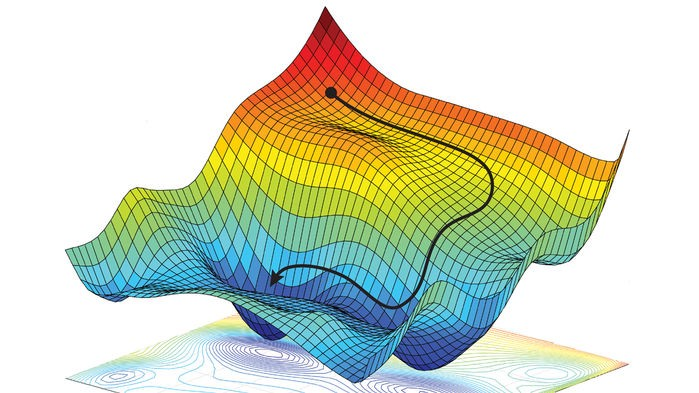
\includegraphics[width=0.8\linewidth]{gradient_descend.jpeg}
    \end{figure}
    {\tiny \color{gray}  Source: \url{https://www.sciencemag.org/news/2018/05/ai-researchers-allege-machine-learning-alchemy}}
\end{frame}

\begin{frame}
    \frametitle{What are Kernels?}
    Let $X \subseteq \mathbb{R}^d$ be an input space. A function $k:X \times X \rightarrow \mathbb{R}$ is called a \textbf{kernel}, if there exists an inner product space $(F, \langle \cdot, \cdot \rangle)$ and a function $\varphi: X \rightarrow F$ which satisfies
    \begin{align*}
        k(x, x') = \langle \varphi(x), \varphi(x') \rangle
    \end{align*}
    for all $x, x' \in X$. This is used to find linear solutions for Problems in $F$ which would not be linearily solvable in $X$.
\end{frame}

\begin{frame}
    \frametitle{Example: Gaussian RBF Kernel}
     $k(x,x') = \textup{exp}(-\frac{{\vert \vert x-x' \vert \vert}_2^2}{h})$ for some $h \in \mathbb{R}$.
    \begin{figure}
        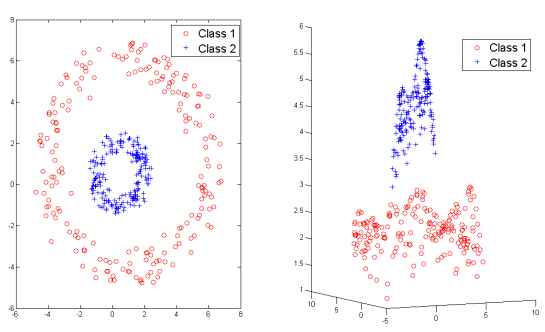
\includegraphics[width=0.8\linewidth]{rbf_kernel.png}
    \end{figure}
    {\tiny \color{gray}  Source: \url{https://i.stack.imgur.com/7yM2K.png
    }}
\end{frame}

\begin{frame}
    \frametitle{What is KL divergence?}
    The Kullback-Leibler (KL) divergence is a measure of how different one continuous probability distribution is from another.
    \begin{align*}
        \textup{KL}(q \vert \vert p) &\coloneqq \int\displaylimits_X p(x) \textup{log}\frac{q(x)}{p(x)} dx \\
        = \int\displaylimits_{x \sim q} \textup{log}\frac{q(x)}{p(x)} dx &= \mathbb{E}_q[\textup{log} \ q(x) - \textup{log} \ p(x)]
    \end{align*}
\end{frame}


%------------------------------------------------
\section{Problem Setup}
%------------------------------------------------
\begin{frame}
    \frametitle{Problem Setup}
    Let $X$ be a continuous random variable taking values in $\mathcal{X} \subseteq \mathbb{R}^d$, $\{D_k\}$ a set of $N$ i.i.d. observations. Then with a prior distribution $p_0(x)$ we have
    \begin{align*}
        p(x \vert \{ D_k\}) = \frac{p_o(x) \prod\limits_{k=1}^{N} p(D_k \vert x)}{\bigintss p_0(x) \prod\limits_{k=1}^Np(D_k \vert x) dx} .
    \end{align*}
\end{frame}


%------------------------------------------------
\section{Stein's Identity}
%------------------------------------------------
\begin{frame}
    \frametitle{Stein's Identity}
    Let $p(x)$ be a smooth density on $\mathcal{X}$, $\phi(x) = [\phi_1(x),...,\phi_d(x)]^T$ a smooth vector function. Then if $\phi$ is sufficiently regular we have
    \begin{align}
        \mathbb{E}_p[\mathcal{A}_p \phi(x)] &= 0, \\ \textup{where} \ \mathcal{A}_p \phi(x) &= \phi(x) \nabla_x \textup{log}p(x)^T + \nabla_x \phi(x). \nonumber
    \end{align}
    $\mathcal{A}_p$ is called the \textbf{Stein Operator} and we say that $\phi$ is in the Stein class of $p$ if (1) holds.
\end{frame}

\begin{frame}
    \frametitle{Stein Discrepancy}
    Consider another smooth density $q(x)$. Then we get a discrepancy measure via
    \begin{align*}
        \mathbb{S}(q,p) = \underset{\substack{\phi \in \mathcal{H}^d \\ \vert \vert \phi \vert \vert \leq 1}}{\textup{max}}\{\mathbb{E}_q[\textup{tr}(\mathcal{A}_p \phi(x))]^2\},
    \end{align*}
    \uncover<2->{
        $\mathcal{H}^d$ being the reproducing kernel Hilbert space (RKHS) for some kernel $k$. The optimal solution has been shown to be
        \begin{align*}
            \phi_{q,p}^*(\cdot) = \mathbb{E}_q[\mathcal{A}_p k(x,\cdot)],
        \end{align*}
        normalized to $\phi(x) = \phi_{q,p}^*(x) / \vert \vert \phi_{q,p}^*\vert \vert $.
    }
\end{frame}

%------------------------------------------------
\section{Algorithm}
%------------------------------------------------

\begin{frame}
    \frametitle{The \textit{variational} Part}
    Given a set of distibutions $\{\mathcal{Q}\}$, we want to approximate the target distribution $p(x)$ by minimizing the KL divergence.
    \begin{align*}
        q^* = \underset{q \in \mathcal{Q}}{\textup{min}} \{ \textup{KL}(q \vert \vert p)\}
    \end{align*}
    \uncover<2->{
    Focus on sets $\mathcal{Q}$ consisting of distributions obtained by transforming a reference distribution. If $T: \mathcal{X} \rightarrow \mathcal{X}$ is a transformation, consider $x \sim q_0$ and $z = T(x)$ with density
    \begin{align*}
        q_{[T]}(z) = q(T^{-1}(z)) \cdot \vert \textup{det}(\nabla_zT^{-1}(z))\vert .
    \end{align*}
    }
\end{frame}

\begin{frame}
    \frametitle{Stein Operator and KL Divergence}
    Let $T(x) = x + \epsilon \phi(x)$ be a transformation, $x \sim q(x)$ and $z = T(x)$ with density $q_{[T]}(z)$. Then
    \begin{align*}
        {\nabla_{\epsilon}\textup{KL}(q_{[T]} \vert \vert p)\vert}_{\epsilon = 0} = - \mathbb{E}_q[\textup{tr}(\mathcal{A}_p\phi(x))].
    \end{align*}
    \uncover<2->{
        We know from earlier
        \begin{align*}
            \phi_{q,p}^* = \underset{\substack{\phi \in \mathcal{H}^d \\ \vert \vert \phi \vert \vert \leq 1}}{\textup{argmax}}\{\mathbb{E}_q[\textup{tr}(\mathcal{A}_p \phi(x))]^2\}.
        \end{align*}
    }
    \uncover<3->{
        So for $T(x) = x + f(x)$, $f \in \mathcal{H}^d$ we have
        \begin{align*}
            {\nabla_{f}\textup{KL}(q_{[T]} \vert \vert p)\vert}_{f = 0} = -\phi_{q,p}^*(x).
        \end{align*}
    }
\end{frame}

\begin{frame}
    \frametitle{The Algorithm}
    $T^*(x) = x + \epsilon \cdot \phi_{q,p}^*(x)$ is equal to a step of functional gradient descend in RKHS. Additionally, we can express $\phi_{q,p}^*$ with respect to our kernel $k$:
    \begin{align*}
        \phi_{q,p}^*(\cdot) = \mathbb{E}_q[k(x,\cdot)\nabla_x\textup{log}p(x) + \nabla_x k(x,\cdot)]
    \end{align*}
    \vskip-0.375em
    \uncover<2->{
        {\centering
        \begin{minipage}{.9\linewidth}
            \begin{algorithm}[H]
                \caption*{}
                \begin{flushleft}
                    \footnotesize
                    \textbf{Input:} Target distribution density $p(x)$, set of initial particles $\{x_i\}_{i=1}^n$. \\
                    \textbf{Output:} Set of particles $\{x_i\}_{i=1}^n$ that approximate the target distribution.
                \end{flushleft}
                \vskip-0.3em
                \begin{algorithmic}[1]
                \small
                \FOR{$\ell=1$ to \textit{max\_iterations}}
                \FOR{$i=1$ to $n$}
                \STATE $x_i^{\ell+1} = x_i^\ell + \epsilon \cdot \hat \phi^*(x_i^\ell)$, \\
                where $\hat \phi^*(x) = \frac{1}{n} \sum\limits_{j=1}^{n} (k(x_j^\ell,x) \nabla_{x_j^\ell} \textup{log} \hskip 0.1em p(x_j^\ell) + \nabla_{x_j^\ell} k(x_j^\ell,x))$ 
                \ENDFOR
                \ENDFOR
                \end{algorithmic}
                \caption{Stein Variational Gradient Descend}
            \end{algorithm}
        \end{minipage}
        }
    }
\end{frame}

\begin{frame}
\frametitle{Examples}
\begin{figure}
    \animategraphics[controls = none, width=0.8\linewidth]{10}{./animation_svgd/svgd_mvn-}{0}{299}
\end{figure}
\end{frame}

\begin{frame}
    \frametitle{Examples}
    \vskip-2em
    \begin{align*}
        {\scriptstyle
        \hat \phi^*(x) = \frac{1}{n} \sum\limits_{j=1}^{n} (k(x_j^\ell,x) \nabla_{x_j^\ell} \textup{log} \hskip 0.1em p(x_j^\ell) + \nabla_{x_j^\ell} k(x_j^\ell,x))}
    \end{align*}
    \vskip-1em
    \begin{columns}
        \begin{column}{.5\textwidth}
            \animategraphics[controls=none, trim = 4cm 0 3cm 0, width=\textwidth]{10}{./animation_grad/grad_mvn-}{0}{199}
        \end{column}
        \begin{column}{.5\textwidth}
            \animategraphics[controls=none, trim = 4cm 0 3cm 0, width=\textwidth]{10}{./animation_kernel/kernel_mvn-}{0}{199}
        \end{column}
      \end{columns}
\end{frame}


\begin{frame}
    \frametitle{The Algorithm}
    Because the update only depends on $\nabla \textup{log} \hskip0.1em p(x)$ and \begin{align*}
        \nabla \textup{log} \hskip0.1em \frac{p(x)}{Z} = \nabla (\textup{log} \hskip0.1em p(x) - \textup{log} \hskip0.1em Z) = \nabla \textup{log} \hskip0.1em p(x),
    \end{align*}
    we can completely ignore the normalization constant. Suddenly,
    \begin{align*}
        p(x \vert \{ D_k\}) = p_o(x) \prod\limits_{k=1}^{N} p(D_k \vert x)
    \end{align*}
    is good enough as an estimator.
\end{frame}
%------------------------------------------------
\section{References}
%------------------------------------------------

\begin{frame}
\frametitle{References}
\footnotesize{
\begin{thebibliography}{99}
\bibitem {}\href{https://arxiv.org/abs/1608.04471}{Liu, Qiang and Wang, Dilin (2016)}
\newblock Stein Variational Gradient Descent: A General Purpose Bayesian Inference Algorithm
\newblock \emph{arXiv} 1608.04471
%--------------------------------------------
\newblock {}{\href{https://github.com/DartML/Stein-Variational-Gradient-Descent}{github.com/DartML/Stein-Variational-Gradient-Descend}}
\end{thebibliography}
}
\end{frame}


\end{document} 